\documentclass[a4paper,12pt]{article}

% 导言区
\usepackage{titlesec}
\usepackage{lipsum} % 示例用,可以删除
\usepackage{geometry}
\usepackage{setspace}
\usepackage{amsmath} % 用于数学公式
\usepackage{graphicx} % 用于插入图片
\usepackage{float}
\usepackage{lipsum} % 用于生成虚拟文本
\usepackage{ctex} % 导入 ctex 包以支持中文
\usepackage{titlesec} % 导入 titlesec 包以定制标题样式
\usepackage{fontspec} % 用于设置中文字体
\usepackage{amsfonts}
\usepackage{amsmath} % 提供 \text 和 \tanh 命令
\usepackage{bm}      % 提供 \bm 命令用于粗体
% 目录设置
\usepackage[nottoc,notlot,notlof]{tocbibind}
\usepackage{enumitem}
% 页面设置
\geometry{margin=1in}

% 标题设置
\titleformat{\section}{\normalfont\Large\bfseries}{\thesection}{1em}{}
\titleformat{\subsection}{\normalfont\large\bfseries}{\thesubsection}{1em}{}
\titleformat{\subsubsection}{\normalfont\normalsize\bfseries}{\thesubsubsection}{1em}{}

% 行间距设置
\onehalfspacing

% 文档信息
\title{项目启动文档}
\author{需求不寄小分队}
\date{\today}

\begin{document}

    \maketitle

% 添加目录
    \tableofcontents

    \section{项目概要}

    \subsection{项目选题}
    一款面向大众的虚拟会议软件,名称TODO
    \subsection{团队成员}
    211250124 程智镝

    211250122 刘辉

    211250159 陈凌

    211250158 李忠信
    \subsection{度量数值}
    本文档共包含TODO个要点与TODO个关联关系,平均要点数量为TODO个。

    要点之间的关联详见第4部分

    \section{项目简介}
    项目旨在帮助用户在任何地点和任何时间进行高质量的在线会议和协作,从各个维度满足用户对于远程会议的需要。通过提供音频、视频、文字聊天、文件共享和屏幕共享等功能来促进沟通和协作。主要目标是提供一个安全、可靠、用户友好的平台,从小型团队会议到大型企业级活动满足各种用户需求。

    项目的根本出发点是基本会议功能。支持用户创建和加入会议,支持同时多人在线会议。允许用户共享他的屏幕,方便在会议中展示演示文稿,应用程序或是其他内容。支持文字聊天,提供实时文本聊天服务,方便在会议期间交流和提问。允许用户单向屏蔽,选择性的不接收来自某人的消息以及音视频聊天。支持会议禁言成员。允许用户设置自动保存会议回放至本地及云端。

    我们新增了日历集成功能,与日历应用程序合作,方便用户安排会议时间并向会议成员发送提醒。添加了会议规划的功能,用户可以查看会议的历史记录,以及将未来的会议添加到会议规划,也就是日历中,在会议开始前会向用户发送提醒,避免遗忘而错过会议。
    为了不错过每次会议的精彩瞬间,我们添加了可以自行选择开关的会议自动备份功能,会议持有者选择开启后,会议成员在申请通过后可以在云端查看此次会议的回放并提供下载到本地的服务。我们提供了文件共享和云存储集成功能,一方面,允许用户在实时会议中发送文件,图片以及文档,方便实时交流和讨论;另一方面,与云存储服务如OneDrive,DropBox集成,便于存储文件和重复查看。

    我们引入了社交系统,对已存在联系人列表中的其他用户,用户可以直接在应用中发出会议邀请,好友会收到入会邀请。我们同时开放了广场功能,即开放的会议室,让会议不只局限于严肃的教学和组会中,尝试将会议功能娱乐化,用户可以在本地或者添加网址链接的方式选择一段音乐或是电影,邀请好友共同观看,或是创建一个公开房间,允许大厅中的陌生人加入你一同听歌或是观影,并可以通过语音,文字实时交流,通过添加好友的功能去开启一段崭新的邂逅之旅吧!同时,类似于公开课之类的学习课程也可以在广场中面向所有有学习需求的用户开放,通过对主题的筛选,用户可以很方便的找到想要加入的公开会议。让会议不再只是熟人之间的工具,也成为陌生人之间分享与沟通的桥梁。

    我们对企业所需求的会议进行了专门的加密隐私处理,提供端到端加密以保护会议内容的隐私安全。通过申请发起企业会议权限,用户可以创建一个更具安全性保密性的会议,首先,加入会议的成员需要通过会议持有者审核才可加入会议,其次,支持多人同时共享,多设备同时操作,让入会者更加高效办公。用户可以与之前提到的日历功能配合使用,预定周期性的会议,不再需要每次提前准备申请企业会议,减少重复操作次数。

    我们针对教育需求新增了教学会议功能,提供了面向线上课堂的专属会议模块,添加了诸如小组讨论,举手答题,课堂小测等功能,课堂回放保存至云端可以随时访问,尽可能地模拟线下课堂的环境,结合线上教学的优势条件,让智能教学更加普及。


    \section{商业模式画布}
    \textbf{画布}
    \begin{figure}[H]
        \centering
        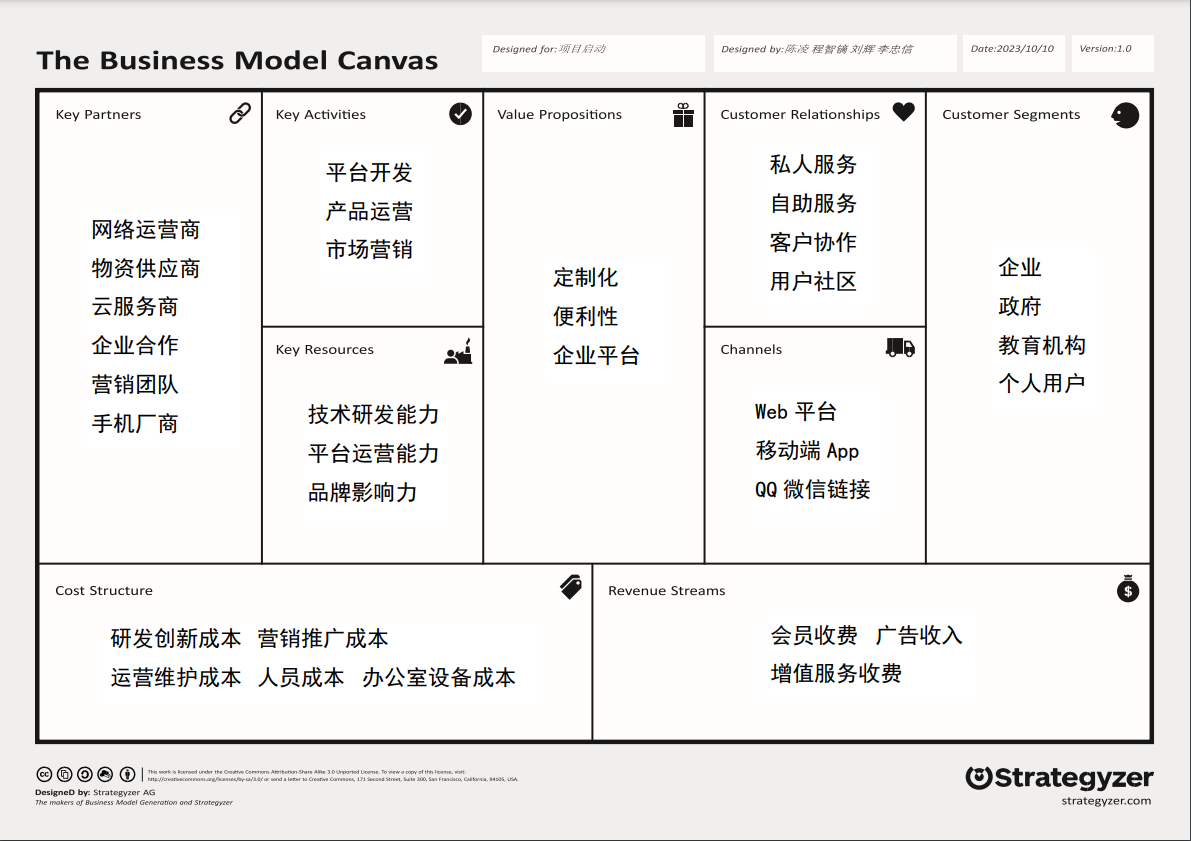
\includegraphics[scale=0.4]{腾讯会议画布.png}
        \caption{腾讯商业模式画布}
        \label{figure}
    \end{figure}

    \textbf{要点讲解}
    \subsection{重要合作}
    \begin{enumerate}
        \item 网络运营商:腾讯会议需要合作网络运营商确保高质量的网络连接,尤其是在视频会议等需要大带宽的场景。
        \item 物资供应商:物资供应商可能提供与硬件设备、办公室设备等相关的支持和服务。
        \item 云服务商:与云服务商的合作有助于提高会议平台的弹性、可伸缩性,并提供高效的存储和计算资源。
        \item 企业合作:合作企业可能提供定制化解决方案、集成服务或其他支持,以满足企业级用户的特殊需求。
        \item 营销团队:营销团队的合作将有助于推广和宣传腾讯会议,吸引更多用户,尤其是企业用户。
        \item 手机厂商:会议软件要通过与手机厂商合作,在其旗下手机产品上预装,扩展用户量,达到宣传的作用。
    \end{enumerate}

    \subsection{关键业务}
    \begin{enumerate}
        \item 平台开发:持续的技术研发和平台开发是确保腾讯会议保持竞争力和技术创新的关键活动。
        \item 产品运营:有效的产品运营确保用户体验优越,功能得到充分利用,并满足不断变化的用户需求。
        \item 市场营销:强大的市场营销活动有助于提高品牌知名度,吸引新用户,尤其是在竞争激烈的在线会议市场。
    \end{enumerate}

    \subsection{核心资源}
    \begin{enumerate}
        \item 技术研发能力:这是腾讯会议成功的核心,需要持续投资并保持领先的技术水平。
        \item 平台运营能力:有效的平台运营确保服务的高可用性、可靠性、稳定性和高效性。
        \item 品牌影响力:强大的品牌影响力可以吸引更多用户,建立信任关系,并为腾讯会议带来竞争优势。
    \end{enumerate}

    \subsection{成本结构}
    \begin{enumerate}
        \item 研发创新成本:高水平的研发投入是必不可少的,以确保平台的不断创新和领先地位。
        \item 运营维护成本:保持平台的稳定性和可用性需要不断的运营和维护工作。
        \item 营销推广成本:在激烈的市场竞争中,持续的营销是必要的,但也需要控制成本。
        \item 人员成本:涵盖研发、运营、营销等方面的人员成本。
        \item 办公室设备成本:包括办公空间、硬件设备等的成本。
    \end{enumerate}

    \subsection{价值主张}
    \begin{enumerate}
        \item 定制化:会议提供诸多细化的可选择性设置。比如可通过选择是否允许回放,是否静音或屏蔽聊天等功能定制自己想要的会议类型。
        \item 便利性:用户可以即使创建快速会议,并且可以通过分享的链接“一键入会”,方便使用。
        \item 企业平台:产品最大限度地在线上满足企业线下活动的条件。针对企业会议,多人共享,讨论组等功能满足了成果展示,面试等基本企业活动所需的条件。更重要的是,长期会议与文件的上传与保存的功能更好的满足了企业的需求。
    \end{enumerate}

    \subsection{客户关系}
    \begin{enumerate}
        \item 私人服务:为个人用户提供个性化的服务和支持。
        \item 自助服务:提供简便易用的自助服务工具,使用户能够更好地管理其会议过程。
        \item 客户协作:与企业客户建立密切的合作关系,以满足其特定需求。
        \item 用户社区:建立用户社区,促进用户之间的互动和信息共享。
    \end{enumerate}

    \subsection{渠道通路}
    \begin{enumerate}
        \item Web平台、移动端App:主要的服务传递渠道,满足用户在不同设备上的需求。
        \item QQ微信链接:通过主流社交媒体渠道进行推广,扩大用户基础。
    \end{enumerate}

    \subsection{收入来源}
    \begin{enumerate}
        \item 会员收费:提供高级会员服务,收取会员费用。
        \item 增值服务收费:提供一些额外的增值服务,如大规模会议、高级安全功能等。
        \item 广告收入:在免费版本中通过广告植入获取收入。
    \end{enumerate}

    \subsection{客户细分}
    \begin{enumerate}
        \item 企业:想要进行线上会议办公的企业用户。
        \item 政府:想要进行线上会议办公的政府机构用户。
        \item 教育机构:想要进行远程沟通授课的学校或教育机构用户。
        \item 个人用户:想要临时召开或者参与线上会议的普通用户。
    \end{enumerate}


    \section{要点关联}
    \subsection{网络运营商与平台开发}\
    \begin{itemize}
        \item \textbf{关联关系:} 网络运营商的合作对于腾讯会议的高质量网络连接至关重要。
        \item \textbf{理由:}一个可靠的、高质量的网络连接是视频会议等服务正常运行的基础,与网络运营商的紧密合作可以确保用户在使用腾讯会议时获得良好的网络体验。
    \end{itemize}
    \subsection{云服务商与平台开发和运营}
    \begin{itemize}
        \item\textbf{关联关系:} 云服务商的合作有助于提高会议平台的弹性、可伸缩性,并为平台提供高效的存储和计算资源。
        \item \textbf{理由:} 会议平台需要应对不同规模的使用和数据存储需求,与云服务商的合作可以使平台更具灵活性和可扩展性。
    \end{itemize}
    \subsection{营销团队与市场营销}
    \begin{itemize}
        \item\textbf{关联关系:} 营销团队是推广和宣传腾讯会议的关键力量,使用户对产品产生兴趣。
        \item\textbf{理由:} 在激烈的市场竞争中,通过有力的市场营销活动,可以提高品牌知名度,吸引新用户,尤其是各大企业用户。
    \end{itemize}
    \subsection{技术研发能力与平台开发}
    \begin{itemize}
        \item\textbf{关联关系:} 技术研发能力是平台开发的核心,支撑着腾讯会议的不断创新和领先地位。
        \item\textbf{理由:} 在快速发展的技术环境中,持续的研发投入可以确保腾讯会议在功能和性能方面保持竞争力。
    \end{itemize}
    \subsection{平台运营能力与客户关系}
    \begin{itemize}
        \item\textbf{关联关系:} 有效的平台运营确保服务的可靠性和稳定性,与客户关系的质量直接关系到用户的满意度。
        \item\textbf{理由:} 用户对于会议平台的可靠性和稳定性有高度的期望,良好的平台运营能力可以增强客户对平台的信任。
    \end{itemize}
    \subsection{会员收费与增值服务收费}
    \begin{itemize}
        \item\textbf{关联关系:} 会员收费和增值服务收费是腾讯会议的主要收入来源,二者之间存在协同关系。
        \item\textbf{理由:} 通过提供高级会员服务和额外的增值服务,腾讯会议可以吸引用户选择付费服务,进而增加收入。
    \end{itemize}
    \subsection{产品运营与客户关系}
    \begin{itemize}
        \item\textbf{关联关系:} 产品运营的质量直接影响用户体验,与客户关系的品质有紧密联系。
        \item\textbf{理由:} 通过有效的产品运营,确保用户的良好体验,用户更有可能对服务保持满意,并可能成为长期忠实用户,增加用户粘性。
    \end{itemize}
    \subsection{广告收入与客户群体}
    \begin{itemize}
        \item\textbf{关联关系:} 广告收入的多寡与吸引不同客户群体的能力密切相关。
        \item\textbf{理由:} 通过了解不同客户群体的需求和兴趣,腾讯会议可以吸引更多广告商,实现广告收入的多元化。
    \end{itemize}
    \subsection{用户社区与客户关系}
    \begin{itemize}
        \item\textbf{关联关系:} 用户社区是客户关系的一部分,对用户社区的建设可以加强用户之间的互动。
        \item\textbf{理由:} 社区提供了一个平台,让用户分享经验、提出建议,加强用户对腾讯会议的参与感,提高用户忠诚度。
    \end{itemize}
    \subsection{增值服务收费与平台开发}
    \begin{itemize}
        \item\textbf{关联关系:} 新的增值服务的推出通常需要平台开发的支持。
        \item\textbf{理由:} 通过不断创新和开发新的增值服务,可以吸引更多付费用户,为腾讯会议带来额外的收入。
    \end{itemize}
    \subsection{企业与客户协作}
    \begin{itemize}
        \item\textbf{关联关系:} 企业是腾讯会议的重要客户群体,与企业的紧密合作可以满足其特殊需求。
        \item\textbf{理由:} 通过与企业合作,提供定制解决方案和集成服务,可以增强腾讯会议在企业市场的竞争力。
    \end{itemize}

    \section{问题域}
    \subsection{用户体验}
    腾讯会议需要登陆才能参加会议,登陆时需要收集很多无关的用户个人信息,让用户感觉隐私受到窥探,体验糟糕。
    \subsection{安全隐私}
    腾讯会议曾被指责存在安全漏洞,使得会议容易受到未经授权的干扰。虽然腾讯已经采取措施改进安全性,但仍然需要不断提高保障用户隐私和数据安全的标准。
    \subsection{网络性能}
    在网络连接不稳定的情况下,腾讯会议有时会出现连接问题,延迟和丢失严重,导致会议质量下降。在低带宽环境下无法稳定进行会议。
    \subsection{移动端性能}
    根据用户反馈得知,虽然腾讯会议专门开发了面向移动端的应用,但一些用户认为在移动设备上的使用不如在桌面端那样流畅,性能十分卡顿。
    \subsection{整合性}
    在竞争激烈的在线会议市场中,用户通常需要多个工具来满足各种需求,如云端保存文件,文档协作等。而腾讯会议尚没有完全将大部分用户的需求整合入应用中。
    \subsection{收费问题}
    目前腾讯会议对于免费用户创建的超过2人的会议限时使用1小时,强迫用户付费使用,对一些用户来说这些成本可能过于昂贵,需要调整收费方案。
    \subsection{社交互动和团队协作}
    在远程工作和协作变得越来越重要的情况下,腾讯会议可以增强社交互动功能,以更好地支持团队协作和沟通需求。
    \subsection{社区}
    腾讯会议未设立社区功能
    \subsection{会议类型}
    腾讯会议没有对用户需求的特定会议进行分类,比如面向课堂的教学会议,面向企业的企业会议等,功能不够齐全
\end{document}
